\documentclass{article}

\title{OpenAI Deep Research --- LaTeX Example}
\author{TODO}
\date{2026-08-24}

\begin{document}
\maketitle

This is a working \textbf{standalone .tex example}. The portfolio converts common article-style LaTeX to its existing safe Markdown/KaTeX reader in the browser.

\section{Math}

Inline probability notation: $p(y\mid x,\theta)$.

\begin{equation}
\operatorname{score}(x) = \sum_{i=1}^{n} w_i f_i(x)
\end{equation}

\section{Lists}

\begin{itemize}
\item Sections and subsections
\item Bold, italic, monospace text
\item Itemized and enumerated lists
\item Simple tabular content
\item Relative figures
\item Inline and display mathematics
\end{itemize}

\section{Simple table}

\begin{tabular}{ll}
Feature & Result \\
Math & KaTeX rendering \\
Image & Relative path resolution \\
Raw source & Always available \\
\end{tabular}

\section{Relative image}

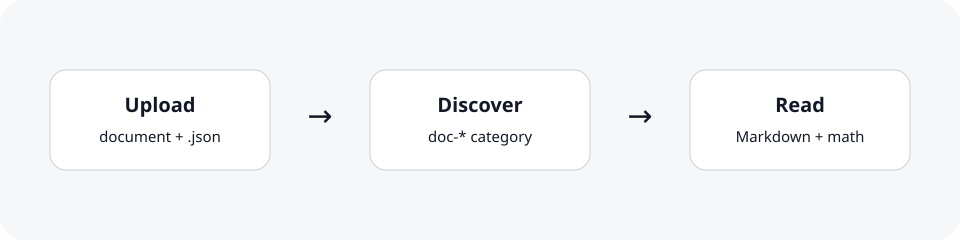
\includegraphics[width=0.9\textwidth]{_assets/example-pipeline.svg}

Complex TeX engine features such as TikZ, arbitrary packages, custom macro expansion, and bibliography compilation intentionally fall back to the \textit{Open raw} source option.

\end{document}
